\chapter{ALE integral assessment scores before and after the mandatory feedback sessions}\label{appendices:scores}

\begin{figure}[h]
    \centering
    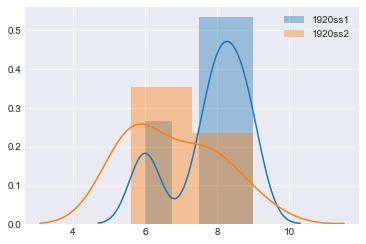
\includegraphics[width=0.7\textwidth]{figures/distribution1920ss.png}
    \caption{\acrshort{ale} integral assessment scores distribution for the 2019-2020 Spring/Summer semester student group}
    \label{fig:distribution1920ss}
\end{figure}
\noindent \Cref{fig:distribution1920ss} shows the score distribution of two data sets, namely 1920ss1 and 1920ss2, where 1920ss is the 2019-2020 Spring/Summer semester \acrshort{ale} group consisting of 19 student from which only 10 students followed \acrshort{ale}1 first then had mandatory feedback sessions in \acrshort{ale}2. 
As the data is skewed (Shapiro-Wilk, $p=0.014$), the non-parametric Wilcoxon signed-rank test was employed at a significance level of 0.05 to test whether there is a significant difference in the performance.
%\\\\
% H$_0$: There is no change, on average, in the performance of 1920ss1 and 1920ss2.\\
% H$_1$: There is an average change in the performance of 1920ss1 and 1920ss2.\\
% Level of significance: $\alpha=0.05$\\
% The test statistic is $t = 45.0$, and $p < 0.05$. 
The resulting $p$-value is smaller than $\alpha=0.05$, thus, the null hypothesis is rejected.\\\\
Although there is significant evidence that the performance changed between 1920ss1 to 1920ss2, according to the distribution, it changed for worse. I believe that enforcing students into showing progress has pushed them to delivering worse quality solution, being pressured to meeting the mandatory feedback sessions deadline.  